% !TEX root = memoire.tex
\begin{introduction}

L'avènement des ordinateurs au cours des dernières décennies a apporté des changements technologiques qui ont bouleversé les communications, la transmission d'informations et le traitement des données numériques. 

En particulier, l'acquisition, la synthèse et le traitement des images constituent  aujourd'hui un champ d'activité fertile pour le développement de nombreuses applications qu'on voit dans la vie de tous les jours. Astronomie, médecine, météorologie, surveillance, vision, sécurité et même le transport sont autant de domaines qui bénéficient de ces avancées technologiques. 

Ces technologies sont basées sur des structures de données et algorithmes opérant sur une matrice de points (pixels) étudiés depuis longtemps et le corpus des connaissances acquises forme le coeur du domaine de la géométrie digitale. On s'accorde généralement pour situer la naissance de ce domaine en 1969 \cite{Rosenfeld69}, bien qu'on trouve des algorithmes pour tracer des segments de droite bien avant \cite{Bresenham65} ainsi que d'autres notions qui se sont avérées équivalentes \cite{Chrl1875}. 

Le plan de pixels s'identifie naturellement au plan discret constitué par le produit cartésien $\Z\times\Z$, et une figure discrète dans le plan n'est rien d'autre qu'un sous-ensemble de $\Z\times\Z$. Les figures connexes dans le plan discret sont commodément représentées par les chemins qui les bornent. Ainsi le bord est constitué par un chemin, ou plusieurs chemins si la figure possède des trous.

Le polyomino est une de ces figures discrètes. Popularisé par S. Golomb~\cite{dbintr39} comme jeu mathématique, le polyomino est un objet combinatoire rencontré dans plusieurs problèmes intéressants tels les pavages~\cite{BN, Golomb} ainsi que certains jeux~\cite{Ga} et problèmes d'énumération~\cite{Jen, JenGutt}. De plus, certaines classes de polyominos codent efficacement les partages d'entiers et sont utilisés en théorie des nombres et en physique mathématique pour représenter le groupe symétrique~\cite{fulton97}. Une représentation commode de tout polyomino est donc réalisée par les chemins qui le bornent.

%Ces objets sont particulièrement étudiés en géométrie digitale et en informatique théorique, les coordonnées entières se prêtant naturellement à l'adressage de composants électroniques distincts bien alignés sur une galette de silicium. 




Ce mémoire concerne deux problèmes importants dans le domaine de la géométrie digitale, à savoir le calcul de l'enveloppe extérieure d'un chemin discret et également la génération exhaustive de polyominos. 



%%%%%%%% Partie chemins %%%%%%%%%%%%
Les objets convexes tiennent un rôle important dans plusieurs branches des mathématiques, comme l'analyse fonctionnelle, l'optimisation, les probabilité et la physique mathématique (voir \cite{Gruber} pour un traitement détaillé de la géométrie convexe et ses applications.) En géométrie euclidienne, étant donné un ensemble fini de points, le problème de trouver le plus petit ensemble convexe les contenant tous a mené à l'introduction de la notion géométrique d'enveloppe convexe. Le calcul de l'enveloppe convexe s'est révélé être l'un des algorithme fondamental de la géométrie computationelle avec des applications allant de la recherche opérationelle \cite{Sherali199483} à l'automatisation du design \cite{kim}. Il est également largement utilisé en graphisme, en particulier dans le traitement d'images \cite{KimLee}. Il est bien connu que dans le cas euclidien, les algorithmes de calcul de l'enveloppe convexe d'un ensemble $S\subset \R^2$ s'exécutent en temps $\O(n\log n)$ où $n=|S|$ (voir \cite{Graham1972132, Chan96}). On peut même montrer que de tels algorithmes sont optimaux à une constante linéaire près \cite{Avis198281,Boas80}.

Néanmoins, en restreignant le problème au calcul de l'enveloppe convexe de polygones simples, une borne asymptotique linéaire est établie  \cite{McCallumAvis, Melkman87}. La version digitale de ce problème est un peu plus compliquée. On peut par exemple calculer l'enveloppe convexe d'un ensemble de pixels $S$ en commençant par calculer l'enveloppe convexe Euclidienne de $S$ et ensuite en digitalisant le résultat \cite{Chaudhuri98}. Ceci nous donne automatiquement un pire cas en $\O(n \log n)$. Dans le cas discret, la situation est surprenamment plus simple grâce à l'aide de la combinatoire des mots, qui a récemment mené au développement d'outils efficaces pour l'étude de la géométrie digitale \cite{thesexavier, blondin12}. Par exemple, des bornes asymptotiques linéaires ont été établues lorsqu'on considère un chemin discret codé par une suite de pas élémentaires. En effet, Brlek et al. ont développé un algorithme linéaire pour calculer l'enveloppe convexe discrète d'un chemin fermé auto-évitant sur la grille carré \cite{blpr09}. Il est basé sur un algorithme de Duval \cite{Duval83} linéaire en temps et en espace optimal pour factoriser un mot de Lyndon. La situation est plus compliquée dans le cas d'un chemin non-simple.

Au chapitre \ref{chapitre-chemins} nous présentons un algorithme linéaire en temps et en mémoire pour calculer l'enveloppe extérieure d'un chemin discret décrit par un mot sur le code de Freeman. L'utilisation d'une structure d'arbre radix augmenté \cite{BKP} permet une représentation linéaire des points visités ainsi que leur liens de voisinage dans le plan discret $\Z \times \Z$. Construire cette structure de données est une opération linéaire en temps et en espace et combinée à l'algorithme de la main droite, bien connu pour la résolution de labyrinthe, permet d'obtenir un algorithme linéaire en temps et en espace pour calculer l'enveloppe externe. Ce résultat fut exposé à la conférence Internationale <<18th IAPR International Conference, DGCI 2014, Siena, Italy, September 10-12, 2014.>>
\begin{quote}\setstretch{0.8} Brlek, S., Tremblay, H., Tremblay, J. et Weber, R. (2014). Efficient computation of the outer hull of a discrete path. Dans Discrete Geometry for Computer Imagery -
 Proceedings, volume 8668 de Lecture Notes in Computer Science. 
\end{quote}

%%%%%%%% Polyominos %%%%%%%%%%%%


%\ref{scamp3}.
 
%\begin{figure}
%\centering
%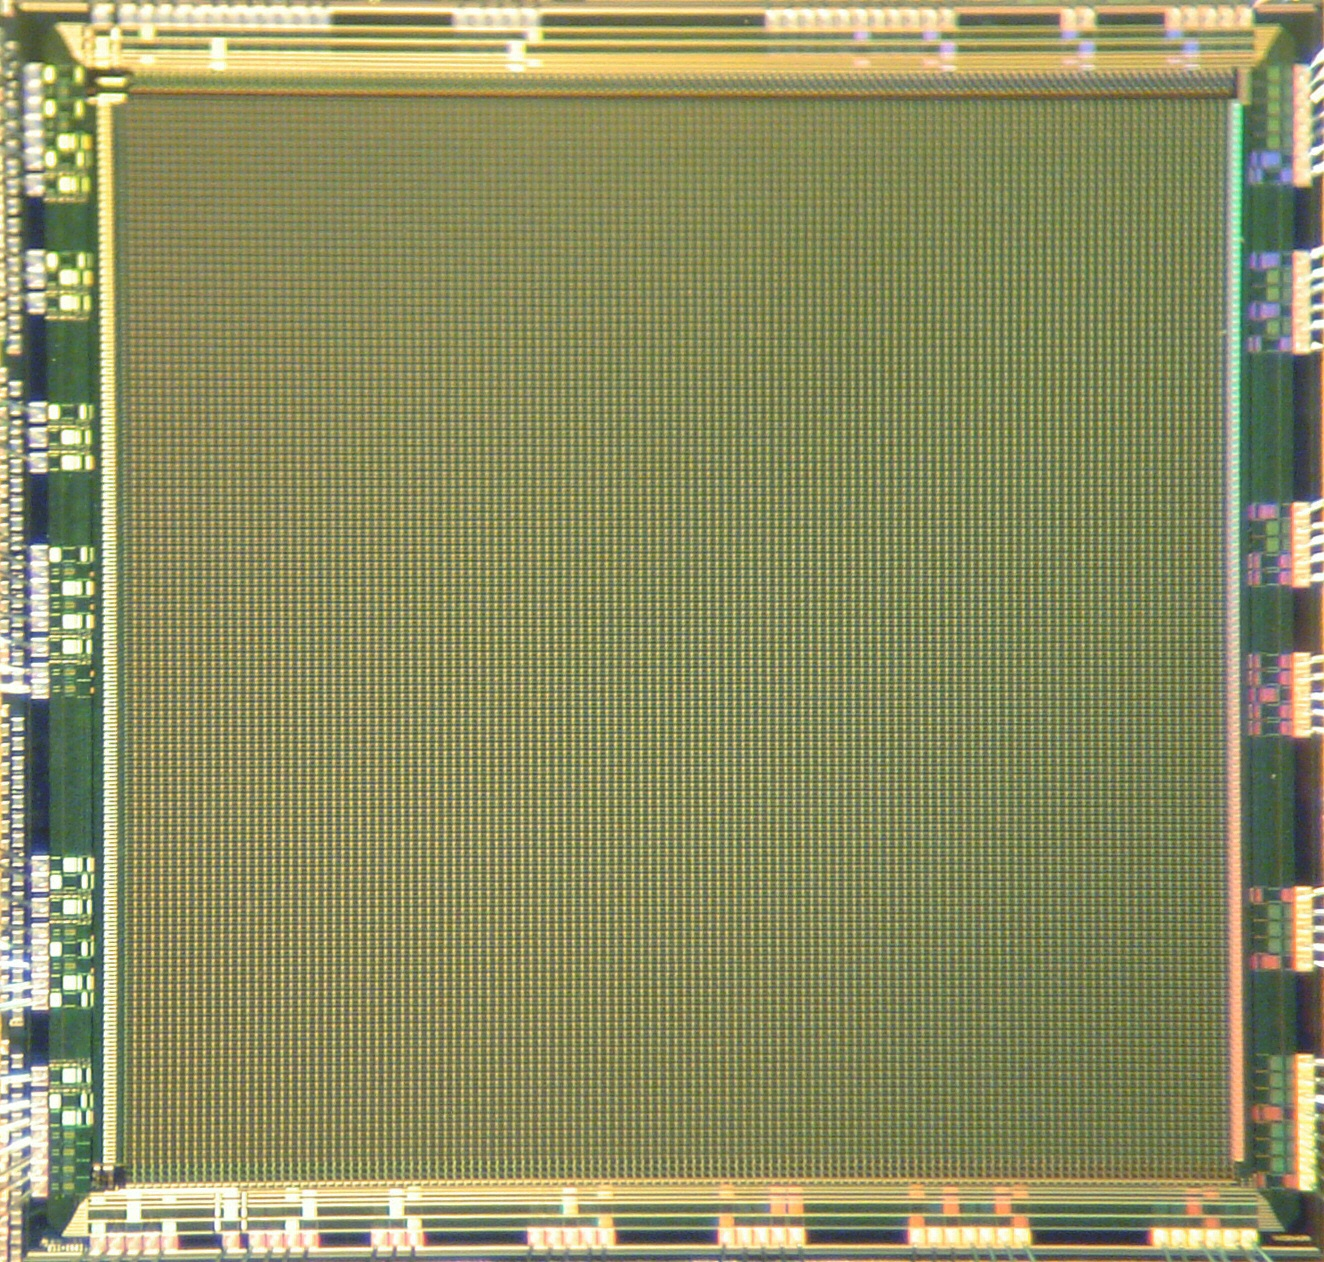
\includegraphics[width=4cm]{scamp3}
%\caption{Le circuit de vision artificielle SCAMP-3 consiste en une grille de $128\times128$ pixels-processeurs\protect\footnotemark.}
%\label{scamp3}
%\end{figure}

%\footnotetext{http://personalpages.manchester.ac.uk/staff/p.dudek/scamp2}

\vspace{-0.5em}
Il existe plusieurs types de polyominos, ceux que nous utiliserons ici sont des ensembles finis de carrés unités connexes par les arêtes dans le plan discret.

\begin{figure}[h]
\centering
\begin{subfigure}[b]{.1\linewidth}
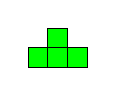
\begin{tikzpicture}[scale=.25, every node/.style={draw, fill=green, rectangle, inner sep=1.25mm}]
\node at (0,0) {};
\node at (1,0) {};
\node at (2,0) {};
\node at (1,1) {};
\end{tikzpicture}
\end{subfigure}
\begin{subfigure}[b]{.1\linewidth}
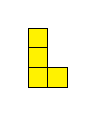
\begin{tikzpicture}[scale=.25, every node/.style={draw, fill=yellow, rectangle, inner sep=1.25mm}]
\node at (0,0) {};
\node at (0,1) {};
\node at (0,2) {};
\node at (1,0) {};
\end{tikzpicture}
\end{subfigure}
\begin{subfigure}[b]{.1\linewidth}
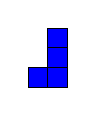
\begin{tikzpicture}[scale=.25, every node/.style={draw, fill=blue, rectangle, inner sep=1.25mm}]
\node at (1,0) {};
\node at (1,1) {};
\node at (1,2) {};
\node at (0,0) {};
\end{tikzpicture}
\end{subfigure}
\begin{subfigure}[b]{.1\linewidth}
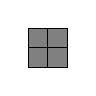
\begin{tikzpicture}[scale=.25, every node/.style={draw, fill=gray, rectangle, inner sep=1.25mm}]
\node at (0,0) {};
\node at (0,1) {};
\node at (1,1) {};
\node at (1,0) {};
\end{tikzpicture}
\end{subfigure}
\begin{subfigure}[b]{.1\linewidth}
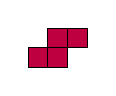
\begin{tikzpicture}[scale=.25, every node/.style={draw, fill=purple, rectangle, inner sep=1.25mm}]
\node at (0,0) {};
\node at (1,0) {};
\node at (1,1) {};
\node at (2,1) {};
\end{tikzpicture}
\end{subfigure}
\begin{subfigure}[b]{.1\linewidth}
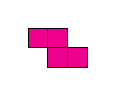
\begin{tikzpicture}[scale=.25, every node/.style={draw, fill=magenta, rectangle, inner sep=1.25mm}]
\node at (0,1) {};
\node at (1,0) {};
\node at (1,1) {};
\node at (2,0) {};
\end{tikzpicture}
\end{subfigure}
\begin{subfigure}[b]{.1\linewidth}
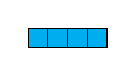
\begin{tikzpicture}[scale=.25, every node/.style={draw, fill=cyan, rectangle, inner sep=1.25mm}]
\node at (0,0) {};
\node at (1,0) {};
\node at (2,0) {};
\node at (3,0) {};
\end{tikzpicture}
\end{subfigure}

\caption{Quelques polyominos $4$-connexes bien connus}
\end{figure}
\vspace{-1.6em}
L'énumération des polyominos en général est un problème difficile encore ouvert. Malgré cela, plusieurs sous-classes ont été énumérées avec succès en imposant différentes contraintes géométriques aux polyominos. Par exemple, il est bien connu~\cite{pol,stan} que le nombre de polyominos parallélogrammes, dont les lignes et les colonnes se croisant sur la diagonale principale sont contigües, de semi-perimètre $(n+1)$ est le $n$-ième {\em nombre de Catalan} (séquence M1459 sur \cite{OEIS}).

\vspace{-0.3em}
En revanche, le nombre $a_n$ de polyominos simplement $4$-connexe sans trous à $n$ cellules a été calculé jusqu'à $n=56$ \cite{Jen,oeisA001168} et le comportement asymptotique du nombre ces polyominos $\left\{a_n \right\}_{n \geq 0}$ est borné par la relation $\lim_{n\rightarrow \infty} \left\{a_n \right\}^{1/n}=\mu$ où \ $3.90 < \mu < 4.64$~\cite{JenGutt,KlarnerRivest}.

\vspace{-0.3em}
Le lecteur qui désire en savoir plus peut consulter Viennot~\cite{Vi} pour l'énumération exacte de plusieurs classes de polyomino, ainsi que \cite{MBM94,MBM96,MBM98} pour plus de résultats, et \cite{BFRV06} pour l'énumération d'une sous-classe de tuiles parallélogrammes. Plus récemment, l'énumération de certaines familles de polyominos inscrits dans un rectangle a été obtenue dans \cite{GCN10}.

\vspace{-0.3em}
Malgré le fait que ces problèmes aient été largement étudiés, plusieurs questions demeurent ouvertes. Par exemple, on ne connaît pas de formule close pour le nombre de polyominos, et la génération presque exhaustive par ordinateur (en utilisant le lemme de Burnside pour prendre en compte certaines symétries) demeure la seule façon de les compter. Plusieurs algorithmes existent tels ceux de Redelmeier \cite{Red}, un algorithme inductif, et celui Jensen \cite{Jen} plus rapide et basé sur les matrices de transfert \cite{stan}. Ces deux algorithmes sont exponentiels, et celui de Jensen gagne en vitesse au prix d'une consommation exponentielle de mémoire.

%%%% Ce mémoire s'intéresse aux polyominos ainsi qu'à quelques algorithmes s'y rattachant. 
\vspace{-0.3em}
Au chapitre \ref{chapitre-generation}, nous exposerons en détail une autre méthode de génération exhaustive, introduite dans \cite{FGLT}, basée sur la contrainte des polyominos selon leur \emph{périmètre de site}~\cite{MBM03,Sieben08}. Le périmètre de site est le nombre de cellules extérieures à un polyomino qui touchent sa bordure. Cet algorithme s'inspire du jeu de go \footnote{https://fr.wikipedia.org/wiki/Go\_(jeu)} et utilise deux types de pierres, noires et blanches. Le résultat présenté ici a fait l'objet de la publication suivante

\begin{quote}\setstretch{1.0}Fortier, J., Goupil, A., Lortie, J. et Tremblay, J. (2013). Exhaustive generation of
gominoes. Theoretical Computer Science, 502, 76--87.
\end{quote}


\end{introduction}